\documentclass{beamer}
\usepackage[ngerman]{babel}
\usepackage[utf8]{inputenc}
\usetheme{Boadilla}

\usepackage{listings}
\usepackage{dirtytalk}
\usepackage{adjustbox}

\begin{document}
\title{Was ist ein Code?}
\subtitle{Grundlagenfach Informatik}
%\subtitle{Freifach Informatik}
%\subtitle{Berufsfeldfach Informatik}
%\subtitle{Ergänzungsfach Informatik}
\author{Oliver Probst (pro@kwse.ch)}
\institute{KSWE}
\date{18. August 2022}
\titlegraphic{
\includegraphics[scale=0.5]{graphics/kswe_logo.pdf}}

\begin{frame}
\titlepage
\end{frame}

\frame{\frametitle{Was ist ein Code?}\framesubtitle{Ampel}
\begin{figure}
\centering
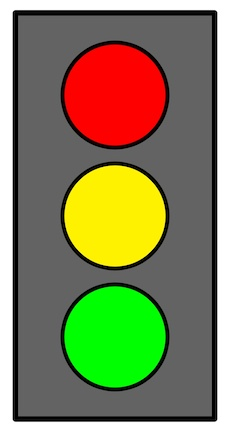
\includegraphics[scale=0.25]{graphics/ampel}
\end{figure}
}

\frame{\frametitle{Was ist ein Code?}\framesubtitle{Energie-Label}
\begin{figure}
\centering
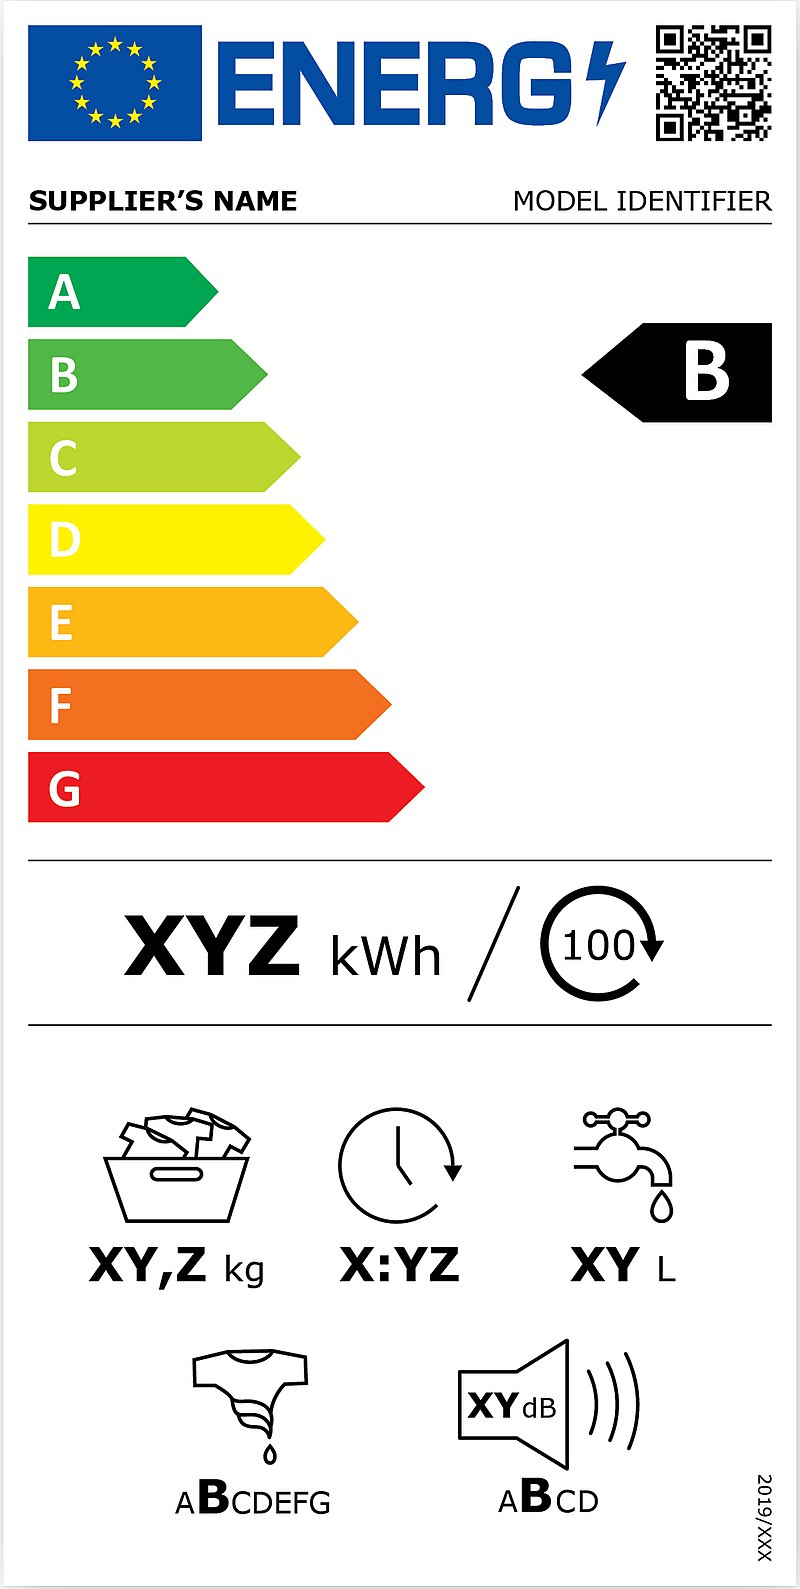
\includegraphics[scale=0.1]{graphics/eu_washing_machines_label}
\end{figure}
}

\frame{\frametitle{Was ist ein Code?}\framesubtitle{Abspielgerät}
\begin{figure}
\centering
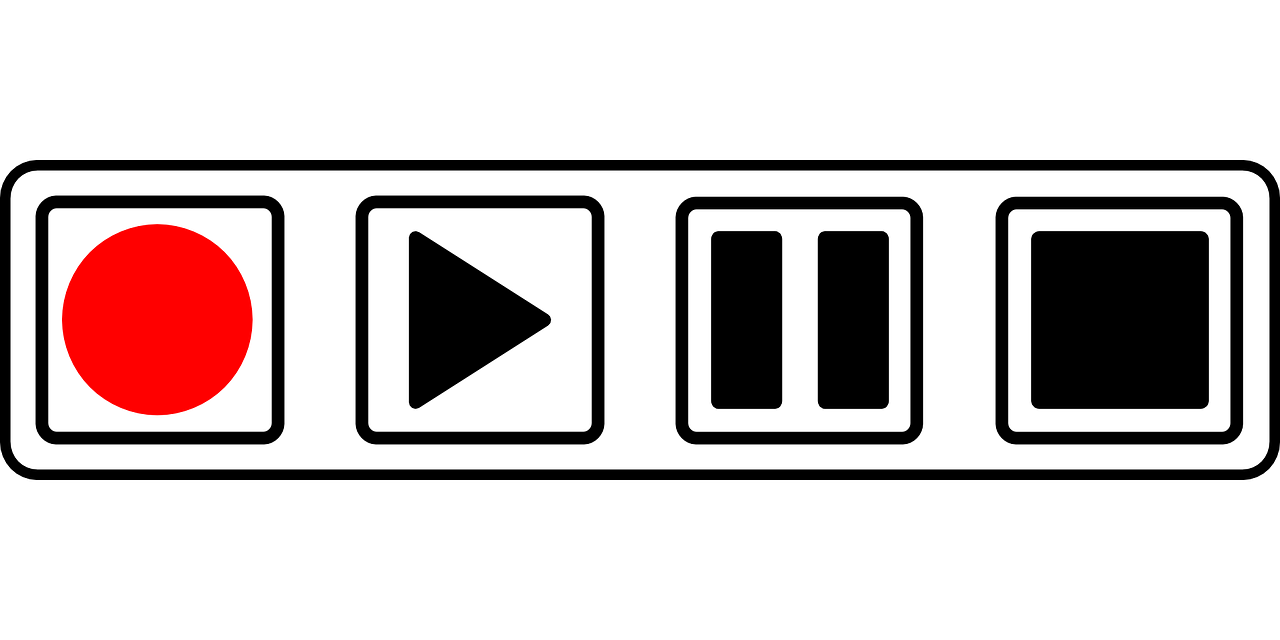
\includegraphics[scale=0.2]{graphics/start_stop_play}
\end{figure}
}

\frame{\frametitle{Was ist ein Code?}\framesubtitle{QR-Code}
\begin{figure}
\centering

\includegraphics[scale=0.2]{graphics/qr_code}
\end{figure}
}

\frame{\frametitle{Was ist ein Code?}\framesubtitle{EAN}
\begin{figure}
\centering
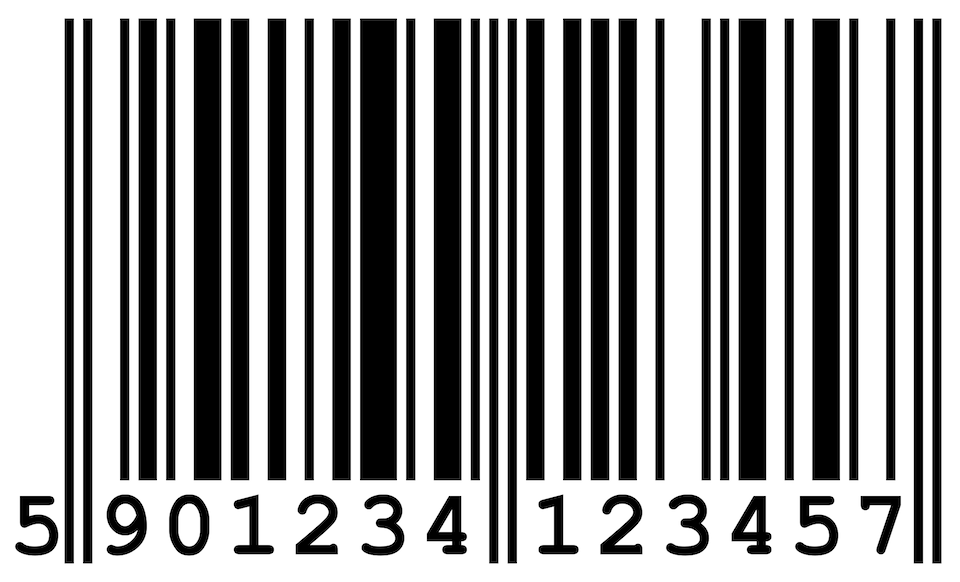
\includegraphics[scale=0.2]{graphics/ean13}
\end{figure}
}

\begin{frame}[fragile]
\frametitle{Was ist ein Code?}\framesubtitle{Unicode}
\begin{figure}
\begin{lstlisting}
01000100 01101001 01100101 01110011 00100000 01101001
01110011 01110100 00100000 01100101 01101001 01101110
00100000 01000010 01101001 01101110 11000011 10100100
01110010 01100011 01101111 01100100 01100101 00101110
\end{lstlisting}
\caption{Leerzeichen und neue Zeilen dienen nur der Übersicht.}
\end{figure}
\end{frame}


\frame{\frametitle{Was ist ein Code?}\framesubtitle{Definition}
Was verstehen wir in der Informatik unter einem Code?
\begin{definition}[Code]
Ein Code ist eine \textbf{Vorschrift}, die beschreibt, wie wir Daten von einer Darstellung in eine andere Darstellung \textbf{umwandeln}. Dabei dürfen keine Daten verloren gehen. Eine eindeutige Rückumwandlung muss immer möglich sein. Die Vorschrift zur Umwandlung kann durch eine \textbf{Code-Tabelle}, eine mathematische Formel oder ein \say{Kochrezept} notiert werden.
\end{definition}
}

\frame[t]{\frametitle{Codes: Morsecode}\framesubtitle{Code-Tabelle}
\begin{table}[htb]
\centering
\begin{adjustbox}{max width=\textwidth}
\begin{tabular}{|c|c||c|c||c|c|}
\hline
\textbf{Zeichen} & \textbf{Code-Wort} & \textbf{Zeichen} & \textbf{Code-Wort} & \textbf{Zeichen} & \textbf{Code-Wort} \\ \hline
A & $\cdot~-$ & J & $\cdot~-~-~-~$ & S & $\cdot~\cdot~\cdot$ \\ \hline
B & $-~\cdot~\cdot~\cdot$ & K & $-~\cdot~-$ & T & $-$ \\ \hline
C & $-~\cdot~-~\cdot$ & L & $\cdot~-\cdot~\cdot$ & U & $\cdot~\cdot~-$ \\ \hline
D &  $-~\cdot~\cdot$  & M & $-~-$ & V & $\cdot~\cdot~\cdot~-$ \\ \hline
E & $\cdot$ & N & $-~\cdot$ & W & $\cdot~-~-$ \\ \hline
F & $\cdot~\cdot~-~\cdot$ & O & $-~-~-~$ & X & $-~\cdot~\cdot~-$ \\ \hline
G & $-~-~\cdot$ & P & $\cdot~-~-~\cdot$  & Y & $-~\cdot~-~-$ \\ \hline
H & $\cdot~\cdot~\cdot~\cdot$ & Q & $-~-~\cdot~-$ & Z & $-~-~\cdot~\cdot~$ \\ \hline
I & $\cdot~\cdot$ & R & $\cdot~-~\cdot$ & @ & $\cdot~-~-~\cdot-~\cdot$ \\ \hline
\end{tabular}
\end{adjustbox}
\caption{Code-Tabelle für den Morsecode. Ein kurzer Ton ist durch einen Punkt dargestellt, ein langer Ton durch einen Strich.}
\label{table-morse}
\end{table}
}

\frame{\frametitle{Codes: Morsecode}\framesubtitle{Decodieren}
Was wurde hier codiert?
\vspace{1cm}
\begin{center}
$\cdot~\cdot~\cdot~~-~-~-~~\cdot~\cdot~\cdot$
\end{center}
}

\begin{frame}[fragile]
\frametitle{Codes: Binärcode}\framesubtitle{Definition}
Was verstehen wir in der Informatik unter einem \textbf{Binärcode}?
\begin{definition}[Binärcode]
Falls ein Code nur Code-Wörter mit den Zeichen $0$ und $1$ verwendet, dann handelt es sich um einen Binärcode.
\end{definition}
Der Satz \say{Dies ist ein Binärcode.} wurde mit dem Binärcode \say{Unicode} wie folgt codiert:
\begin{figure}
\begin{lstlisting}
01000100 01101001 01100101 01110011 00100000 01101001
01110011 01110100 00100000 01100101 01101001 01101110
00100000 01000010 01101001 01101110 11000011 10100100
01110010 01100011 01101111 01100100 01100101 00101110
\end{lstlisting}
\caption{Leerzeichen und neue Zeilen dienen nur der Übersicht.}
\end{figure}
\end{frame}

\end{document}